\documentclass[landscape]{article}
\usepackage[pdftex]{graphicx,color}
\pagestyle{empty}
\oddsidemargin  -0.5 in
\evensidemargin -0.5 in
\headheight     0 in
\topmargin      -1 in
\textheight     7.7 in
\textwidth      10 in
\begin{document}
\Large
\renewcommand{\labelitemi}{-}
\setlength{\parindent}{0 cm}

\mbox{ }

\vfill

\begin{center}
  \Huge Trigger Mystery!
\end{center}

\vspace{-1 cm}

\begin{tabular}{p{0.7\linewidth} p{0.3\linewidth}}
  \begin{minipage}{\linewidth}
    \begin{center}
      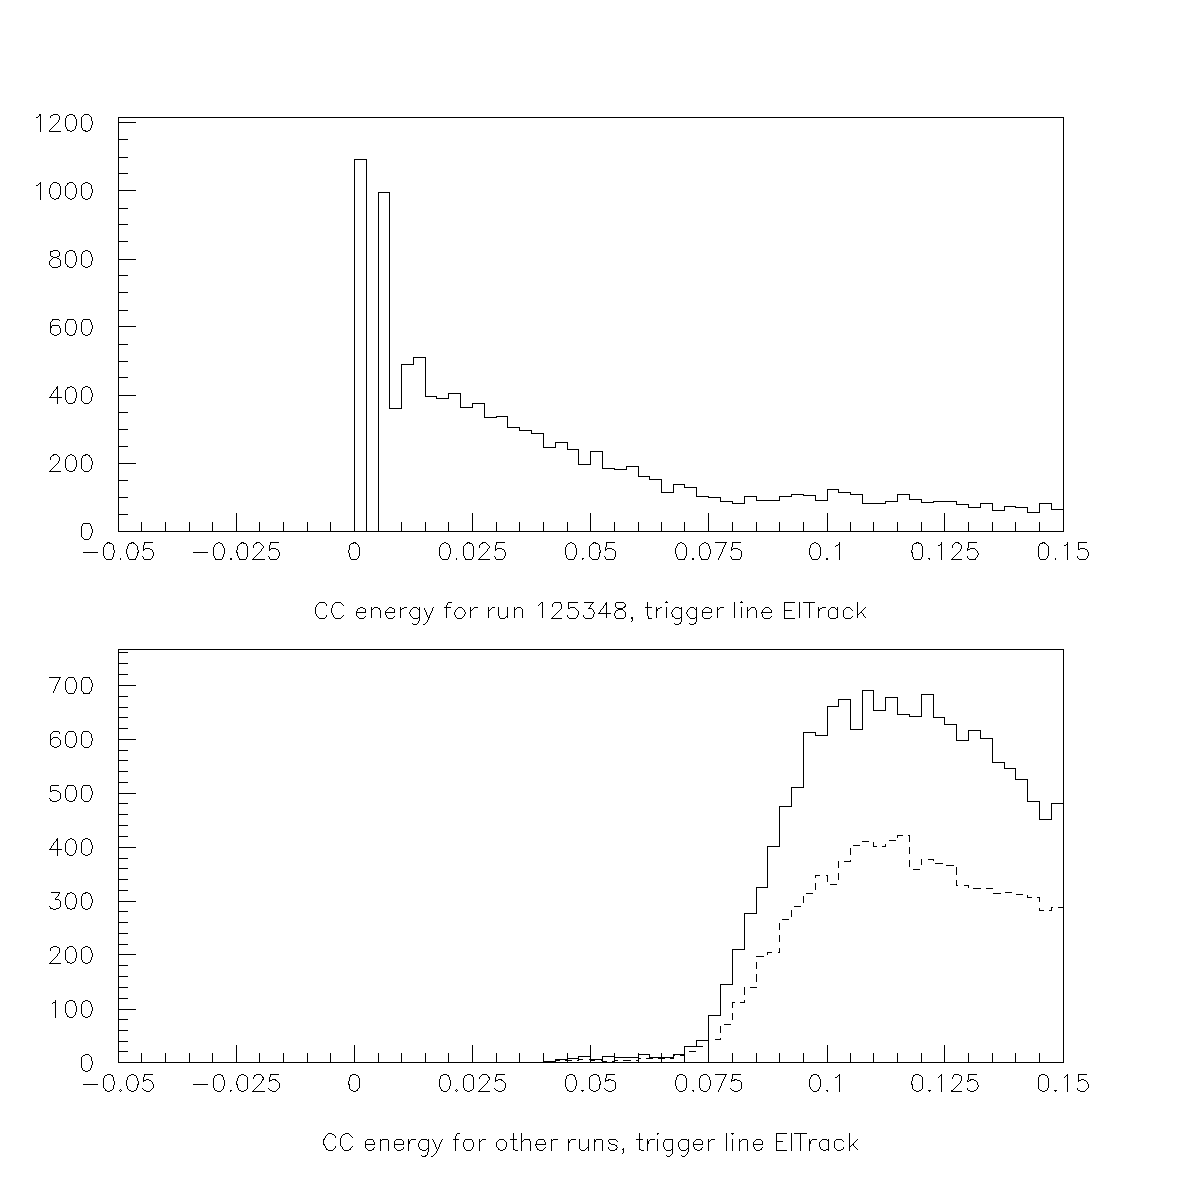
\includegraphics[width=\linewidth]{tr2_nether_eltrack.pdf}
    \end{center}
  \end{minipage} &
  \mbox{\hspace{-1.5 cm} \begin{minipage}{\linewidth}

    This is a trigger malfunction I encountered when looking at raw
    data: run 125348 has many events that passed the ElTrack line with
    at least one CBMD shower.  However, a full reconstruction of the
    event shows that there is not enough energy in the entire CC to
    make the CBMD shower.

    \vspace{0.25 cm} 
    (No cuts were applied to this plot except for the ElTrack trigger.
    It is raw data that came from tape.)

    \vspace{0.25 cm}
    CBMD is not the only variable affected; the CC energy of events
    passing the Hadron line had a different spectum, too.

    \vspace{0.25 cm}
    A list of affected runs is on the next page.

  \end{minipage}} \\
\end{tabular}

\vfill

\pagebreak

\begin{tabular}{p{0.5\linewidth} p{0.3\linewidth}}
  \mbox{\hspace{-0.75 cm} \begin{minipage}{\linewidth}
    \begin{center}
      \includegraphics[width=\linewidth]{/cdat/dafe/mccann/acceptance/wierd_trigger_3.pdf} \\
      \includegraphics[width=\linewidth]{/cdat/dafe/mccann/acceptance/wierd_trigger_3lumi.pdf} \\
    \end{center}
  \end{minipage}} &
  \mbox{\hspace{-1 cm} \begin{minipage}{\linewidth}
      \begin{tabular}{c c c | p{0.001 cm} | c c c}
	run & frac & (nb$^{-1}$) & & run & frac & (nb$^{-1}$) \\\hline
	121595 & 0.0629676 & 1498.9   & &  125348 & 0.0236059 & 297.7 \\	  
	121714 & 0.0186295 & 560.7    & &  126647 & 0.0924731 & 12.7 \\	  
	122330 & 0.0972059 & 1866.1   & &  127026 & 0.0467418 & 510.4 \\	  
	122331 & 0.199991 & 175.0     & &  127028 & 0.0353018 & 268.3 \\	  
	122335 & 0.143708 & 105.4     & &  132221 & 0.0489149 & 1778.2 \\	  
	122336 & 0.198272 & 569.1     & &  132236 & 0.109944 & 1788.1 \\	  
	122339 & 0.199762 & 561.4     & &  132239 & 0.0117223 & 512.3 \\	  
	122341 & 0.202276 & 473.6     & &  132247 & 0.0912106 & 1811.9 \\	  
	122342 & 0.202954 & 360.5     & &  110945 & 0.0903118 & 844.0 \\	  
	122344 & 0.222128 & 50.6      & &  111355 & 0.0215249 & 1638.9 \\	  
	122345 & 0.209215 & 96.3      & &  111357 & 0.0684584 & 766.8 \\	  
	122347 & 0.207477 & 397.0     & &  111361 & 0.0332281 & 480.7 \\	  
	122349 & 0.204689 & 546.0     & &  111578 & 0.133685 & 180.1 \\	  
	122350 & 0.206655 & 553.7     & &  111579 & 0.142677 & 100.2 \\	  
	122351 & 0.203038 & 430.0     & &  111581 & 0.0787731 & 304.2 \\	  
	122352 & 0.205154 & 118.0     & &  111582 & 0.0450814 & 477.0 \\	  
	122353 & 0.55646 & 6.3        & &  112342 & 0.0353313 & 1209.4 \\	  
	124012 & 0.0151013 & 1995.2   & &  112348 & 0.211926 & 422.5 \\      
      \end{tabular}

  \end{minipage}} \\
\end{tabular}





\end{document}
